\chapter{Evaluation}\label{Evaluation}
\ifpdf
    \graphicspath{{Chapter4/Chapter4Figs/PNG/}{Chapter4/Chapter4Figs/PDF/}{Chapter4/Chapter4Figs/}}
\else
    \graphicspath{{Chapter4/Chapter4Figs/EPS/}{Chapter4/Chapter4Figs/}}
\fi
A number of different clustering and classification algorithms have been used in our implementation of the event extraction system. 
Some of them are more suitable for mining social media content and some others are not. In this capter we evaluate quantitatively these algorithms 
based on real data collected from Twitter and we present the results of several experiments we have conducted using this dataset. 
Our quantitative analysis consists of comparing the accuracy and the quality of the clusterers and classifiers as well as their runtime performance. 
Finally, based on our results we discuss and explain which algorithms pass the test and will be used in the development of the proof-of-concept application in Chapter \ref{Pythia}.

\section{Document clustering evaluation}
Cluster analysis is the core component of our system and its evaluation is of great importance to us. We have implemented 
four different clustering algorithms and some of them have been used with success in traditional document clustering. However,
in our case we are asked to tackle an entirely different problem since we deal with social media content and the challenges that come with it. 
We have identified three major challenges that are inherent to tweets and our clustering evaluation evaluates quantitatively the individual merits and demerits 
of each algorithm with respect to these challenges. More specifically, the three major challenges are:

\begin{itemize}
   \item \textbf{Number of documents:} The first difference between traditional document clustering is that our system must operate on a vast amount 
   of tweets. In March 2011 Twitter reported that a billion tweets are sent per week \citep{TwitterBlog} and events that are getting a lot 
   of traction, such as the Arab Spring, will be associated with a huge number of tweets. Therefore, our first consideration is scalability and whether our algorithms can cope with the 
   number of tweets.    
   \item \textbf{Document length:} Tweets, unlike normal web documents, are very short and they are limited to 140 characters. Longer documents are, in general, more likely
  to contain more examples of the features of interest than shorter ones \citep{doi:10.1080/09296174.2011.533588} hence clustering may be more accurate with longer documents. This fact may 
  affect the accuracy of our algorithms and we should investigate their relative performance. In our evaluation we use the notion of average document length which is the sum of lengths of all documents 
  in the corpus divided by the number of documents. 
   \item \textbf{Vocabulary diversity :} Another major challenge due to the nature of the tweets is the diversity of the vocabulary used. Tweets are supposed to be informal documents
   and this greatly affects the quality of their content. For example, many tweets contain spelling mistakes, typos or abbreviations and sometimes users use words from multiple languages.
   Usually people tend to make small modifications to existing tweets and retweet them with the consequence that we collect several tweets that essentially have the same meaning but their
   vocabulary varies. This is a big concern for us since our clustering methods use the vector space representation which utilises the word frequencies to find similarities. Hence the vocabulary 
   diversity will affect the term frequencies and consequently our results. We define vocabulary diversity as the number of distinct terms in a corpus divided by the number of documents in the corpus.
\end{itemize} 
What we try to achieve in the next sections is to evaluate our clustering algorithms by considering the three challenges described above as our variables. We vary these variables and 
record the performance of each algorithm in each case. In addition to these variables we also investigate the effect of different similarity measures on our results. 

   
\subsection{Data and evaluation methodology}\label{ClusteringEvaluationMethod}
Our aim is to measure the quality of a clustering algorithm and we have a few methods to choose from to achieve this. There are two categories of clustering evaluation methods and the choice depends
on whether a ground truth is available. The first category is the extrinsic methods which require the existence of a ground truth and the other category is the intrinsic methods. In general, extrinsic methods try to assign a score, $Q(C, C_g)$, to a clustering $C$, given the ground truth $C_g$, whereas intrinsic methods evaluate clustering by examining how well the clusters are separated and how compact they are \citep{han2005}.\\\\ 
In our evaluation we decided to use an extrinsic method by constructing the ground truth using data from the Arab Spring. More specifically, we use the BCubed precision and recall metrics. The BCubed precision and recall metrics differ from the traditional precision and recall (described in section \ref{ClassifiersEvaluationMethod}) in the sense that clustering is an unsupervised learning technique and therefore we do not know the labels of the clusters beforehand. For this reason BCubed metrics evaluate the presicion and recall for every example in a clustering on a given dataset according to the ground truth. The precision of an example is an indication of how many other examples in the same cluster belong to the same category as the example. The recall of an example reflects how many examples of the same category are assigned to the same cluster.\\\\ 
Formally, let $D = \{ o_1,....,o_n \}$ be a set of examples, and $C$ be a clustering on $D$. Let $L(o_i)$ where $1 \leq i \leq n$ be the label of $o_i$ given by the ground truth, and $C(o_i)$ be the cluster identifier of $o_i$ in $C$. Then, for two examples, $o_i$ and $o_j$, where $i \neq j$, the \emph{correctness} of the relation between $o_i$ and $o_j$ is defined by:

\begin{eqnarray}
Correctness(o_i, o_j) = \begin{cases}
                          1& \text{if $L(o_i) = L(o_j) \Leftrightarrow C(o_i) = C(o_j) $},\\
                          0& \text{otherwise}.
                        \end{cases}
\end{eqnarray} 

BCubed precision is defined as 

\begin{eqnarray}
Precision BCubed = \frac{ \sum_{i=1}^{n} \frac{\sum_{o_j:i \neq j, C(o_i)=C(o_j)}^{} Correctness(o_i, o_j)}{\Vert \{ o_j | i \neq j, C(o_i) = C(o_j)  \}  \Vert} }{n}
\end{eqnarray} 

BCubed Recall is defined as

\begin{eqnarray}
Recall BCubed = \frac{ \sum_{i=1}^{n} \frac{\sum_{o_j:i \neq j, L(o_i)=L(o_j)}^{} Correctness(o_i, o_j)}{\Vert \{ o_j | i \neq j, L(o_i) = L(o_j)  \}  \Vert} }{n}
\end{eqnarray} 
While recall and precision can be used to determine the quality of a classifier, the usual approach is to combine the recall and precision rates in a single equation and this is 
achieved using the $F$ metric which is defined as:
\begin{eqnarray}
F = \frac{2 \times precision \times recall}{precision + recall}
\end{eqnarray} 
    
\subsection{Results}
For the construction of the ground truth we have manually labelled/categorised 285 tweets according to the events they described. In this dataset we have identified 35 different events. These tweets are collected using our data retrieval module and they are related to the Egypt's uprising. More specifically, these tweets describe the events that took place, in Egypt, during a 2-hour period (12pm - 14pm) on 25th of January 2011.    

\subsubsection{Clustering quality vs Number of documents in the dataset}\label{EvalDiffNoDocs}
In this section we investigate the performance of the four different algorithms when the number of documents in our dataset varies while the other variables, the document length and the vocabulary diversity are kept constant. More specifically, we start with a small dataset of 50 documents and we iteratively add more documents (5 each time) until we reach a dataset size of 285. The average document length is $116.44$ characters/document and the vocabulary diversity is $1.17$ words/document. Also, the optimal parameters for the four classifiers are:

\begin{itemize}
  \item \textbf{k-Means:} The number of clusters, $k$, is set to 35 since we expect 35 events to be found. 
  \item \textbf{DBSCAN:} The two parameters needed for DBSCAN are set to $\epsilon=0.5$ and $min\_pts=5$. 
  \item \textbf{NMF:} The number of bases is 35 since we expect 35 events.
  \item \textbf{Online:} The window size is set to one third of the dataset size at any iteration. 
\end{itemize}\vspace{15pt}
We run three different experiments, each one with a different similarity metric. The results we obtained are illustrated in Figure \ref{DifferentSizeResults}

\begin{figure}[htbp]
  \begin{center}
    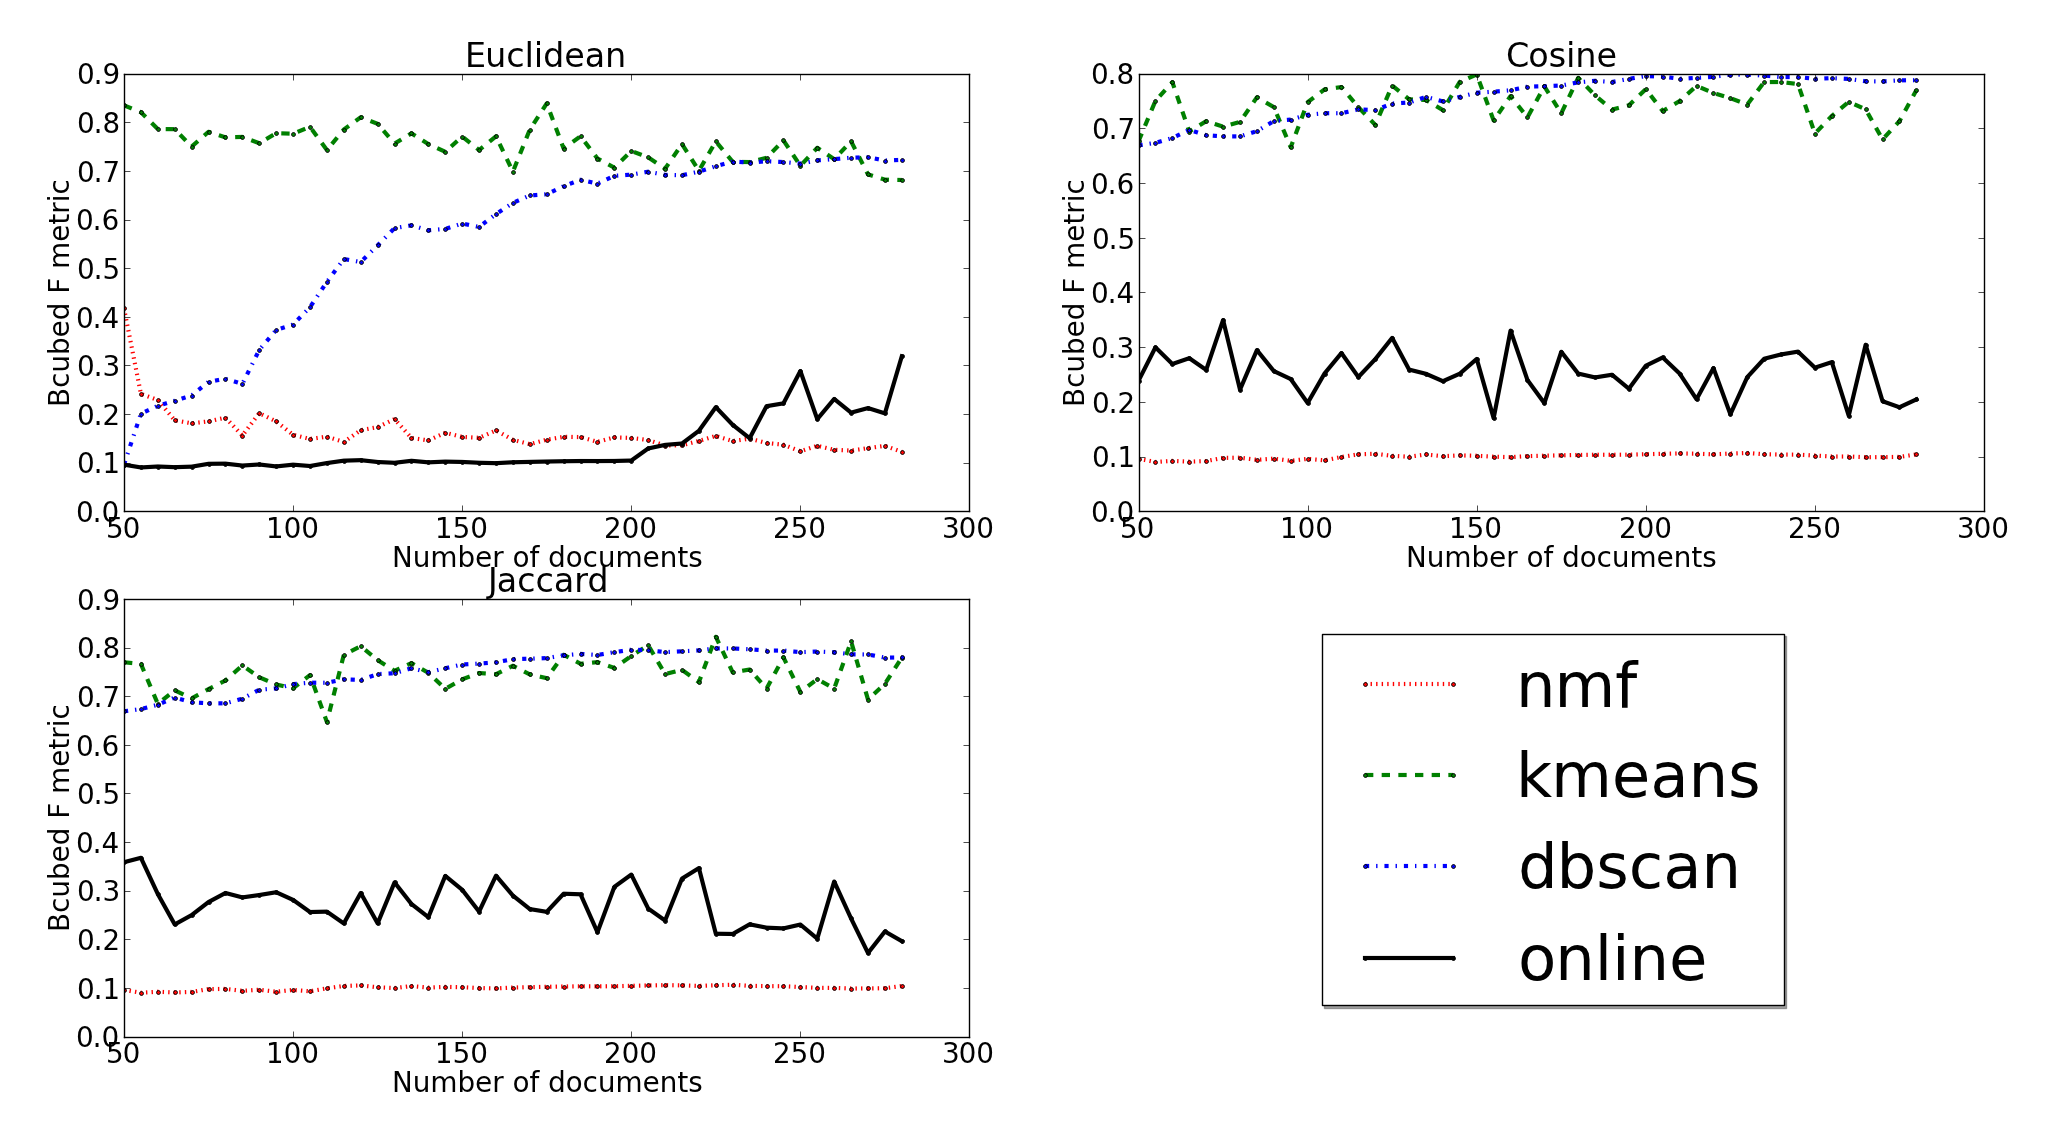
\includegraphics[height=5in, width=6in]{number_of_documents}
    \caption{Each plots depicts the results obtained using a different similarity metric. In each plot we illustrate the BCubed F metric (y-axis) against the number of documents (x-axis) of each clusterer.}
    \label{DifferentSizeResults}
  \end{center}
\end{figure}

\noindent The first important observation is that in all the plots DBSCAN and k-Means clusterers outperform the others in terms of the BCubed F metric. In all three cases k-Means performance is constantly around 0.75 although in the case of Euclidean distance the performance has a slightly negative trend as the number of document increases. On the other hand, DBSCAN initially has very low performance but as the number of documents increases the performance becomes better. A possible explanation is offered in \citep{Pratap2011} which states that a disadvantage of DBSCAN algorithm is that it cannot cluster datasets with large differences in density very well. Initially, the dataset is not very dense since the number of documents is small. However, as the number of document increases the performance increases too. The same scenario is depicted in the cases of cosine and Jaccard similarities. The only difference is that this time the initial performance of DBSCAN is not as low as for the Euclidean case.\\\\
The performances of the other two clusterers are much lower, with the NMF clusterer having the lowest performance. The lower performance of the online clusterer is expected since we have sacrificed accuracy for execution time performance by considering a limited window size. We have mentioned before that the term-frequency matrix for an online clusterer is constructed using only the last $N$ documents where $N$ is the window size. Therefore, any documents before this are lost and the TF-IDF weightings in the matrix are not accurate. A possible solution would be to use an approach similar to a moving average where the new TF-IDF weightings are calculated efficiently based on all the previous information plus the new information coming into the system.   

\subsubsection{Clustering quality vs Average document length}
In this experiment our aim is to evaluate our clusterers by varying the average document lengths of the corpus. We try to emulate the cases when a dataset contains short documents and when it contains very long documents. Also, we want to find what happens in between these two cases. The motivation behind this experiment is that Twitter corpora are very short and we hypothesise that short documents yield worse results in terms of clustering quality.\\\\
We start with our original dataset which is described above and we incrementally add more words in the documents to deliberately increase their length. However, we have to keep the other two variables of our experiments constant. The number of documents is constant at 285 documents and in order to keep the vocabulary diversity constant, at $1.17$ words/document, the words that are appended to the documents are words that already belong to the dataset. Therefore, we achieve an increase in the document length without changing the vocabulary diversity. The initial value for the average document length is $116.44$. The clusterers use the same parameters as in Section \ref{EvalDiffNoDocs}. Again we have run three experiments with each one using a different similarity measure.\\\\  
\begin{figure}[htbp]
  \begin{center}
    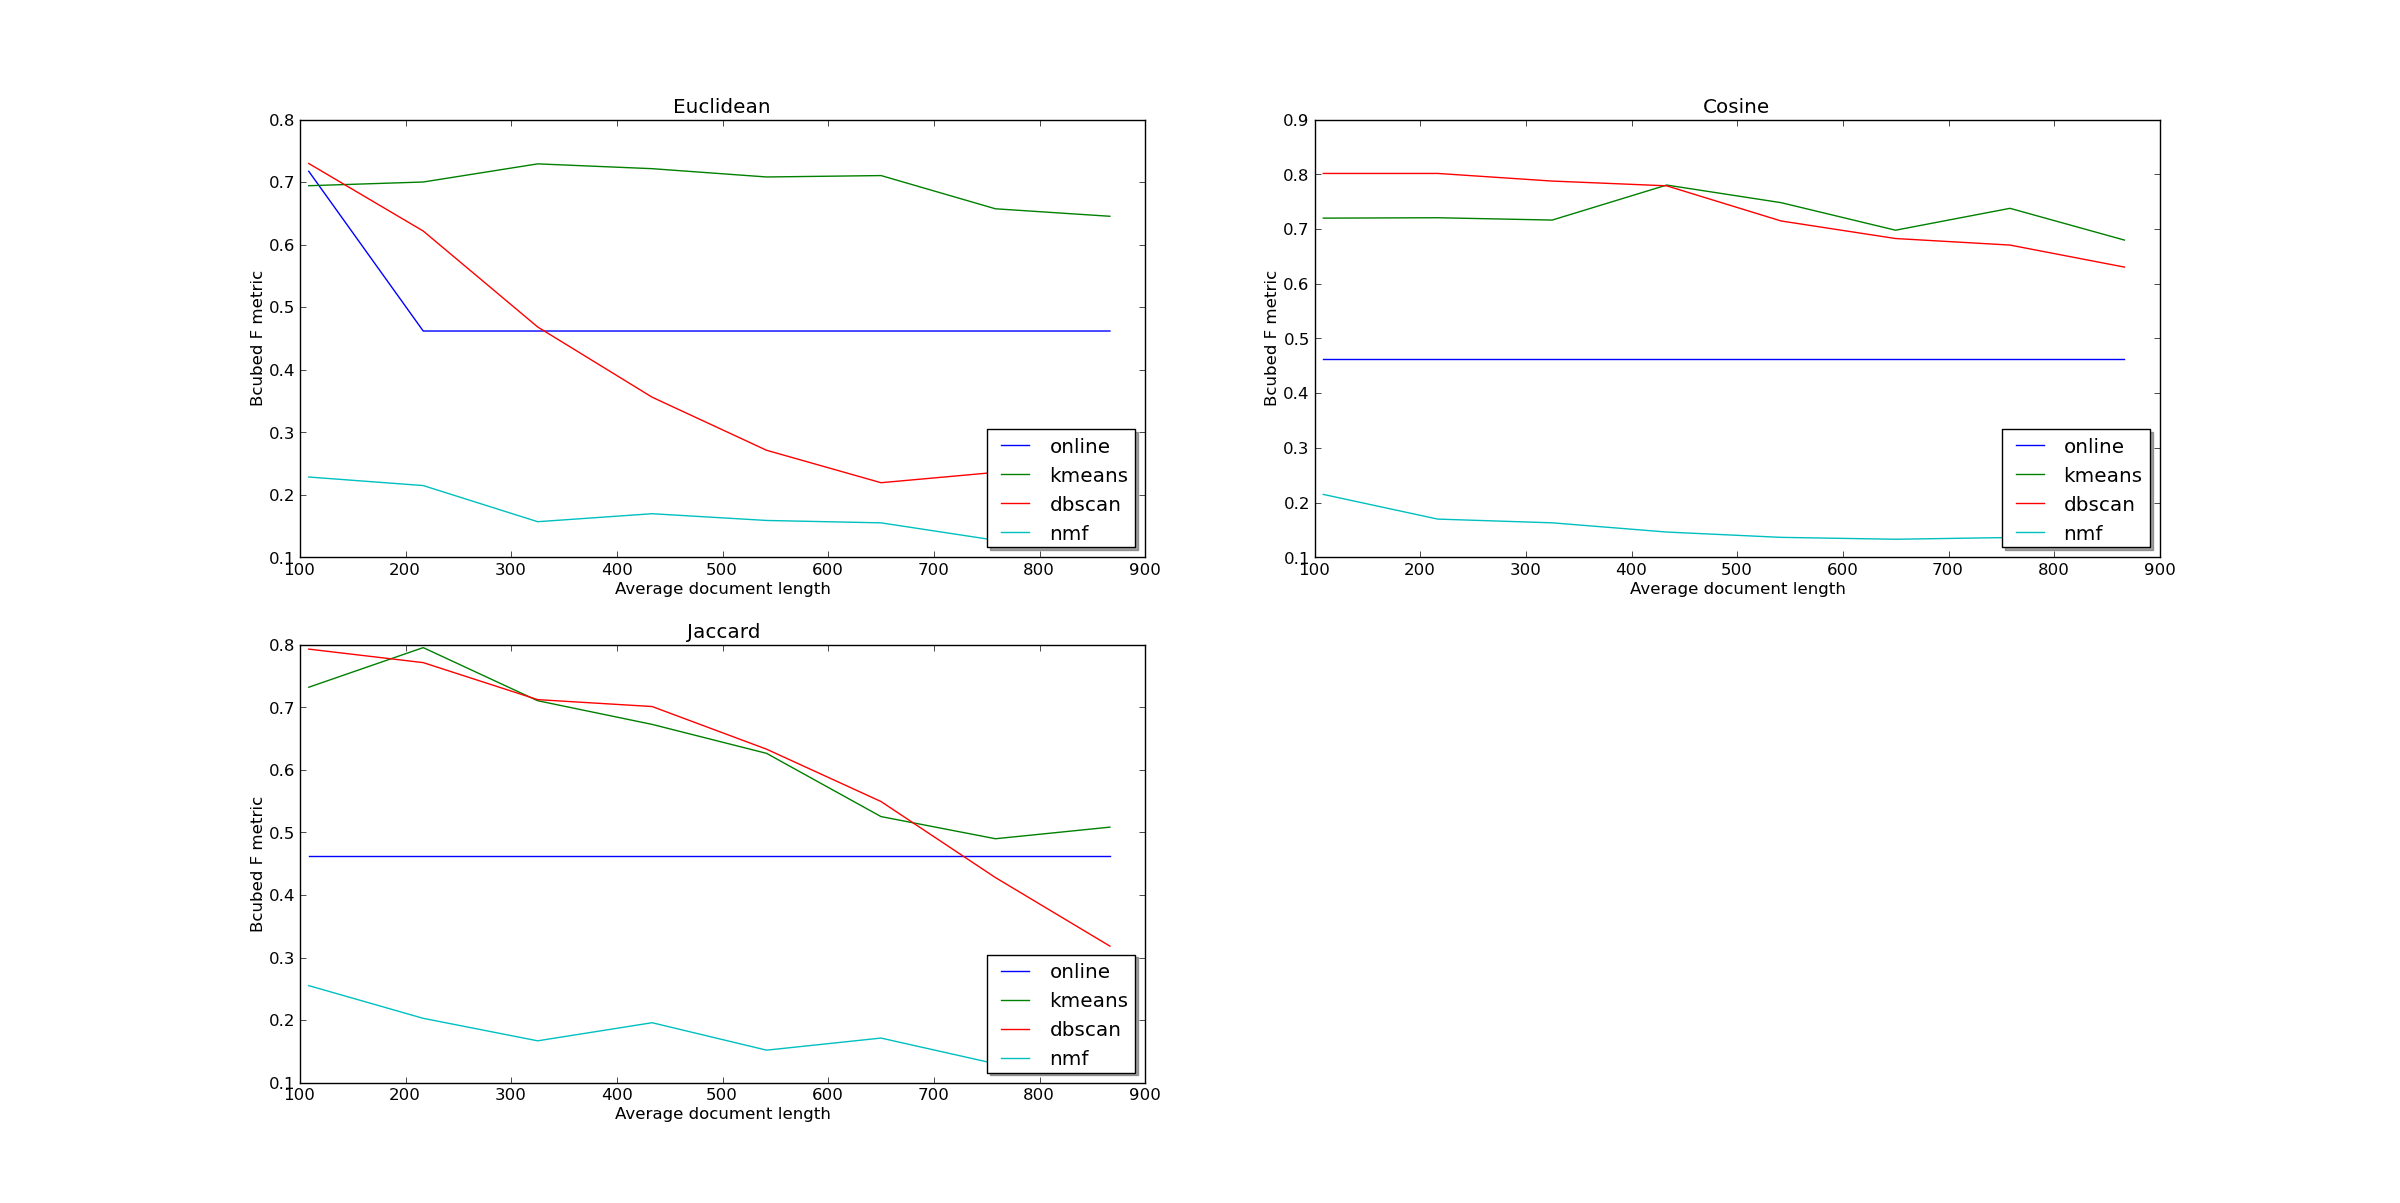
\includegraphics[height=5in, width=6in]{average_document_length}
    \caption{Each plots depicts the results obtained using a different similarity metric when the average document length is varying. In each plot we illustrate the BCubed F metric (y-axis) against the number of documents (x-axis) of each clusterer.}
    \label{DifferentLengthResults}
  \end{center}
\end{figure}

\noindent The results show that the performance of the classifiers is not greatly affected by the average document length. This was not expected as our hypothesis was that longer documents will aid the clustering process. It turns out that in our case the performance remains almost the same and in some cases exactly the same. However, we can clearly see that DBSCAN has the highest BCubed F score except for large document lengths in the Euclidean plot. The next best performing clusterer is k-Means and then online and NMF clusterers are once again inferior in performance.    

\subsubsection{Clustering quality vs Vocabulary diversity}
The final experiment is concerned with vocabulary diversity which is the number of distinct words in a dataset over the number of documents in it. Twitter corpora have a large vocabulary diversity due to the fact that they contain typos, spelling mistakes and abbreviations. In order to fabricate datasets with variable number of vocabulary diversity we employ a dictionary of the English language. More specifically, we begin with our original dataset and in the next iteration we replace some of the words in the documents by random English words starting from a letter in the alphabet. In the next iteration we replace the words with others from the set of words starting from 2 distinct letters of the alphabet. This process continues, increasing the vocabulary diversity each time until we use all the 26 letters of the English alphabet. Also, notice that we remove a small number of the words in the original documents in order to keep the average document constant at $116.44$. The number of documents also remains constant at 285 documents. The parameters for the clusterers are the same as in Section \ref{EvalDiffNoDocs}. The results for the three different similarity measures are shown in Figure \ref{DifferentVocabularyResults}.\\\\ 
\begin{figure}[htbp]
  \begin{center}
    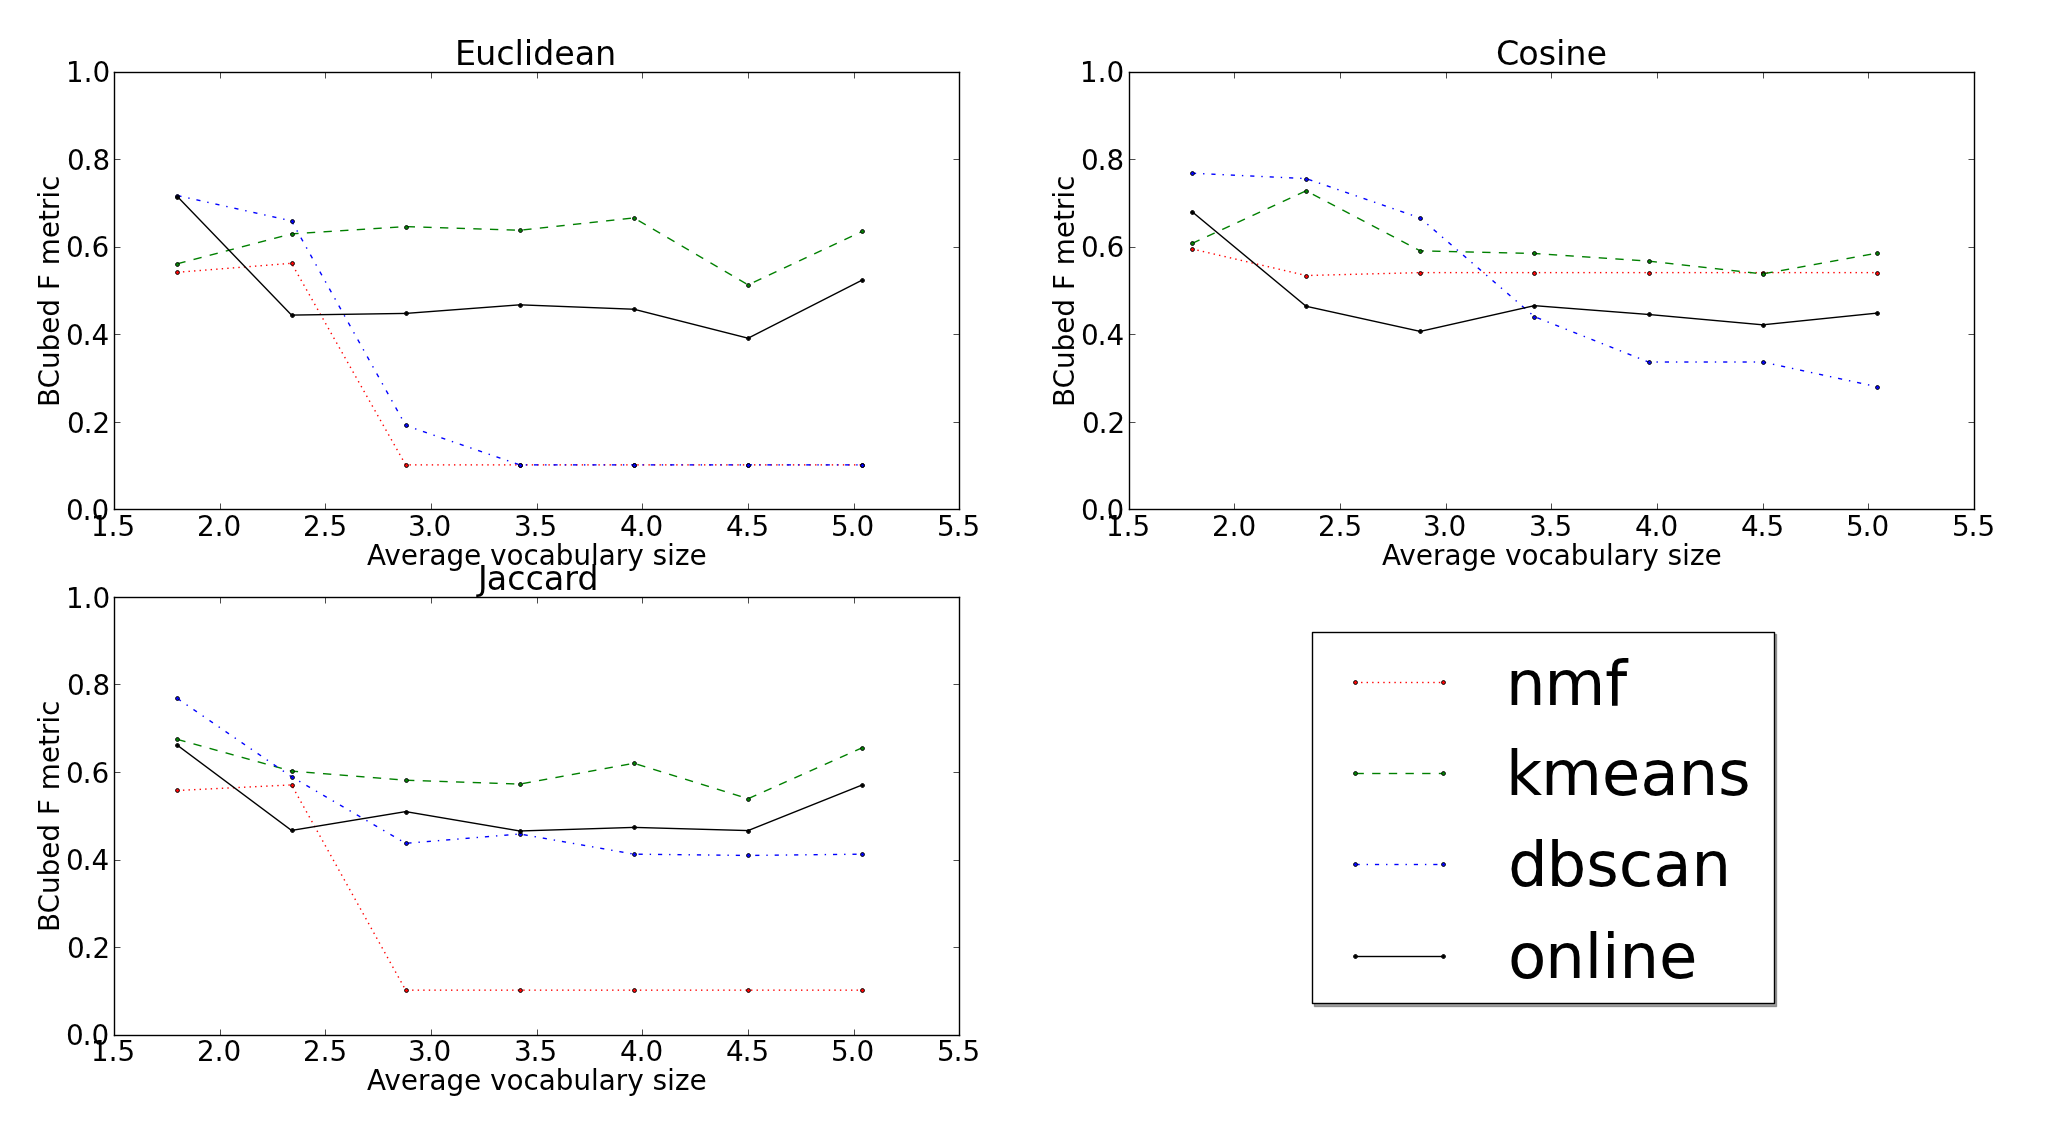
\includegraphics[height=5in, width=6in]{vocabulary}
    \caption{Each plots depicts the results obtained using a different similarity metric. In each plot we illustrate the BCubed F metric (y-axis) against the vocabulary diversity (x-axis) of each clusterer.}
    \label{DifferentVocabularyResults}
  \end{center}
\end{figure}
A first look at the results reveals that k-Means algorithm has the higher BCubed F scores than the other three algorithms. Unlike the other experiments, DBSCAN now has lower performance than online clustering for large vocabulary diversities. The performance of the online clustering is less prone to the effects of large vocabulary diversity whereas the performance of DBSCAN is initially high but it degrades very quickly. The overall trend in the plots indicates that in general as the vocabulary diversity increases the BCubed F score decreases for all clusterers, except from NMF's score which remains almost constant. An increase in vocabulary diversity means that it is harder to compute similarities between the documents since their common features are fewer and the vectors become sparse. However, in the case of the cosine similarity we can see that the average performance of the clusterers is slightly higher than in the other cases. The reason might be that due to the very diverse vocabulary the term-frequency vectors are very long and sparse and they contain many 0 values. Unlike the Euclidean distance, cosine similarity ignores these 0 values and focuses only on the common words between two documents and thus leads to better results.\\\\
The lower performance in this experiment stems from the fact that the feature vectors are getting larger due to the vocabulary diversity. Therefore, the dimensionality of the space becomes bigger and bigger and the effects of the "curse of dimensionality" reduce the performance of our clusterers. There are some remedies for this problem and one of them is to reduce the dimensionality using feature selection methods. One of these methods is Principal Component Analysis (PCA) which searches for $k$ $n-dimensional$ orthogonal vectors that can best be used to represent the data, where $n$ is the dimensions of the feature vector and $k < n$ \citep{han2005}. We have used Orange's package for PCA and we have applied this dimensionality reduction method on the k-Means and DBSCAN clusterers. The results are shown in Figure \ref{DifferentVocabularyPCAResults}.\\\\ 
\begin{figure}[htbp]
  \begin{center}
    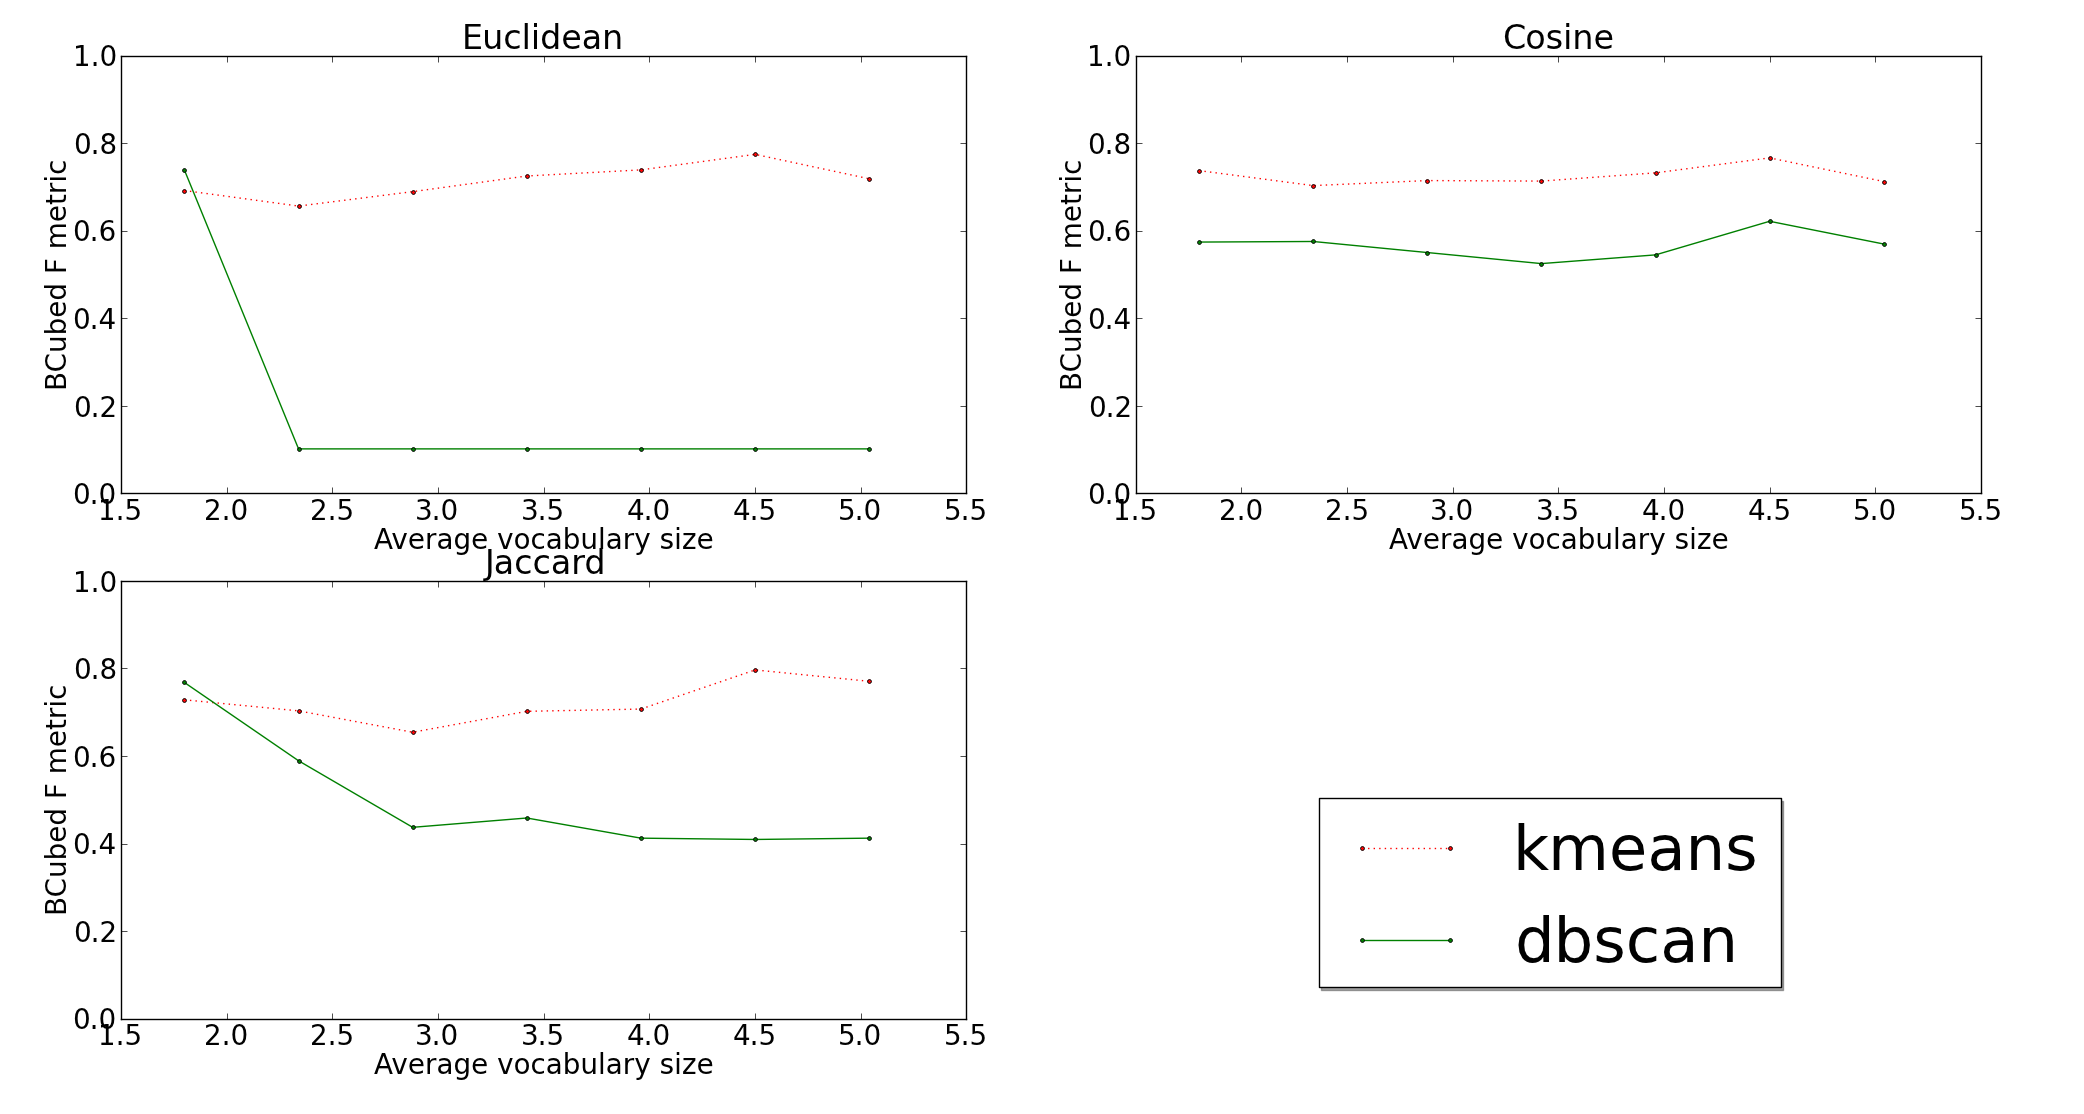
\includegraphics[height=5in, width=6in]{vocabulary_pca}
    \caption{The results for the BCubed F score against the vocabularty diversity after PCA have been used to reduce the dimensionality.}
    \label{DifferentVocabularyPCAResults}
  \end{center}
\end{figure}
\noindent The results are positive since the BCubed F score of k-Means has not only risen but it demonstrates a positive trend in all cases. DBSCAN's score remains the same for the Euclidean and Jaccard cases but it is improved for the case of cosine similarity. The initial score might be lower than the previous case but it never falls below $0.5$. Therefore, PCA can help in this case especially for k-Means.

\subsubsection{Execution time performance}
\begin{center}
\begin{tabular}{ | l | l| l | l | }
  \hline
  \textbf{Clustering method} & \textbf{Euclidean} & \textbf{Cosine} & \textbf{Jaccard} \\ \hline
  k-Means \begin{tabular}{ | r  }  Number of documents  \\ Document Length \\ Vocabulary Diversity \end{tabular} & 1 & 2 & 3 \\
  DBSCAN  \begin{tabular}{ | r  }  Number of documents  \\ Document Length \\ Vocabulary Diversity \end{tabular} & 1 & 2 & 3 \\
  NMF     \begin{tabular}{ | r  }  Number of documents  \\ Document Length \\ Vocabulary Diversity \end{tabular} & 1 & 2 & 3 \\
  Online  \begin{tabular}{ | r  }  Number of documents  \\ Document Length \\ Vocabulary Diversity \end{tabular} & 1 & 2 & 3 \\
  \hline
\end{tabular}
\end{center}

\section{Twitter user classification evaluation}

\subsection{Evaluation methodology}\label{ClassifiersEvaluationMethod}
In this section our aim is to identify which one of our classification algorithms performs better in terms of classification accuracy. Our classifier evaluation process involves the precision and recall metrics as well as the $F_1$ score. The precision and recall metrics definitions in this section are different from the ones described in section \ref{ClusteringEvaluationMethod} since classification is a supervised learning method and we can calculate these metrics using the labels of the training dataset. More specifically, precision can be thought as a measure of what percentage of examples that are classified by a classifier in a certain class are actually members of that class. On the other hand, recall is a measure of what percentage of the overall population of examples, belonging to a certain class, have been classified in that particular class. Formally, precision and recall are defined as:

\begin{eqnarray}
precision = \frac{TP}{TP + FP}
\end{eqnarray}  

\begin{eqnarray}
recall = \frac{TP}{TP + FN}
\end{eqnarray}  

where 

\begin{itemize}
  \item True Positives ($TP$): These are the positive tuples that were correctly labelled by our algorithm. 
  \item True Negatives ($TN$): These are the negative tuples that were correctly labelled by our algorithm.
  \item False Positives ($FP$): These are the negative tuples that were incorrectly labelled as positive by our algorithm.
  \item False Negatives ($FN$): These are the positive tuples that were incorrectly labelled as negatives by our algorithm.
\end{itemize}\vspace{15pt}

\subsection{Results}

In order to carry out our evaluation we have crawled 200 user profiles from Twtrland and labelled them manually according to the five user categories (celebrities, media organisations, journalists, activists and common people). During the process of labelling we made sure that the training dataset was as unambiguous as possible. However, in some cases the choice was not clear especially for the journalists and activists, since these two categories both overlap. Some journalists are known to be activists as well. Finally, in order to produce as accurate results as possible we have used 10-fold cross validation. Cross-validation is the statistical practice of partitioning a sample of data into subsets such that the classifiers accuracy is tested on a single subset, while the other subsets are used for training. Since we have used 10-fold cross validation we split our dataset in subsets of 20 examples and 180 are used for training while the rest are used to test the classifier.\\\\
Figure \ref{DifferentClassifiersResults} demonstrates the average results of running 10-fold cross validation 100 times. Information gain is used as the statistical measure for selecting tree nodes in ID3 and post-pruning of the trees takes place after training in order to minimise the effects of overfitting. Also, for the k-nearest neighbour algorithm we have used Euclidean distance to measure similarity between examples and $k=10$ (10 nearest neighbours have given the best results in our dataset). 
\begin{figure}[htbp]
  \begin{center}
    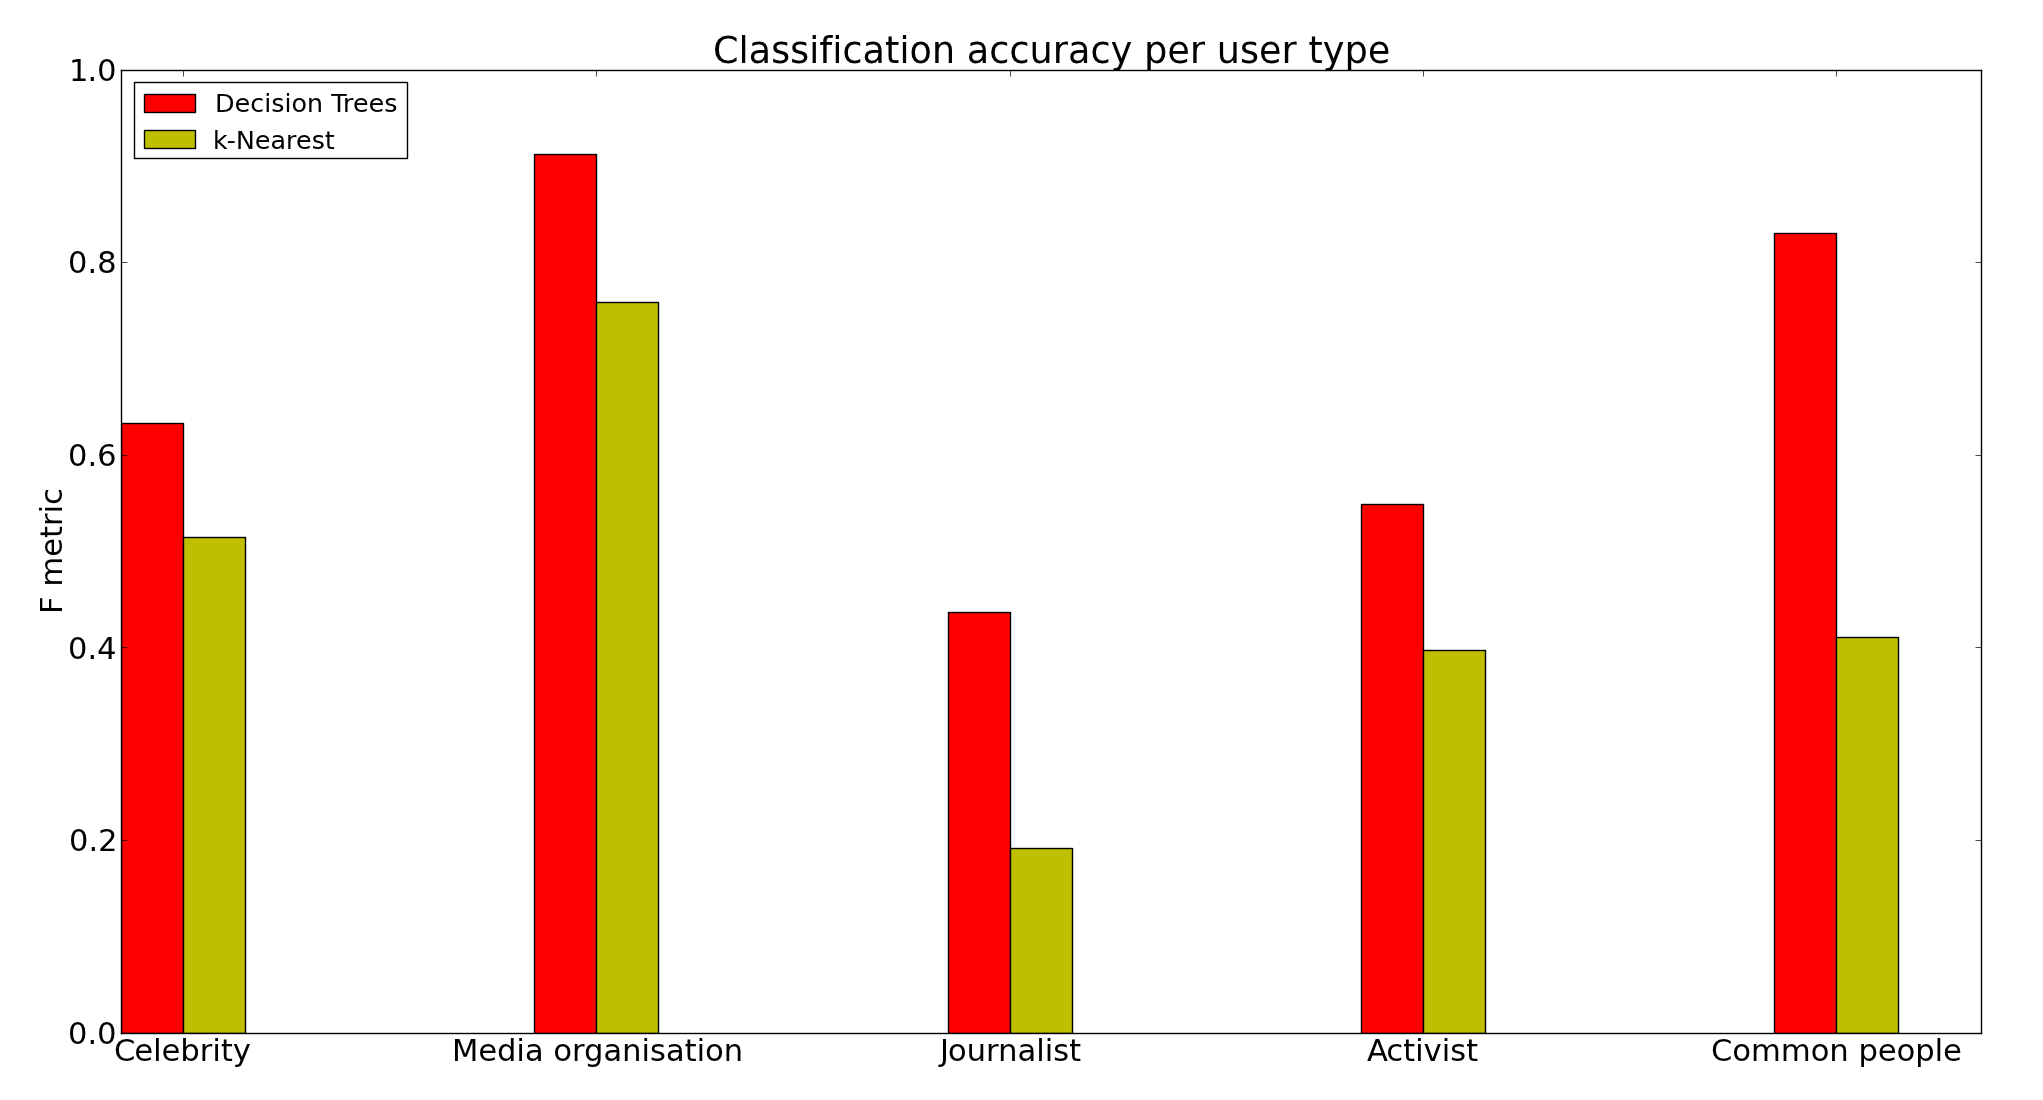
\includegraphics[height=5in, width=6in]{classifiers_bad}
    \caption{The F metrics obtain after 10-fold cross validation on our dataset for the two classifiers. The x-axis depicts the five user types and the y-axis indicates the $F_1$ score of each classifier.}
    \label{DifferentClassifiersResults}
  \end{center}
\end{figure}
The results reveal that for all the classes the performance of the decision tree learning algorithm is better compared to the k-nearest neighbour learning. We attribute the differences in the results in two factors. First of all k-nearest neighbours algorithm is highly effective in cases when it is given a sufficient amount of training data. In our case we have provided a small amount of training examples. The second problem is that since the user feature vectors are constructed based on a user's activity on Twitter we expect to have some outliers indicating irregular activity from some users (i.e. a celebrity having a small followers-to-followees ratio because they follow back almost everyone). These outliers can reduce the performance of a k-nearest neighbour classifier but we can use a weighted version of the algorithm where the effect of distant examples is reduced. Additionally, unlike decision trees, the classification decision is based on all the attributes of the feature vector (Euclidean distance uses the whole vector length to calculate the distance). However, usually only a subset of these attributes is relevant for classification and therefore a similarity measure based on many irrelevant features might be misleading.\\\\ 
Based on the hypothesis that distance-weighted nearest neighbour algorithm can improve the performance we have changed our implementation to take into account the weights of each neighbour and the results are shown in Figure \ref{DifferentClassifiersResultsImproved}. It is obvious that the effect of outliers was significant in the case of common people since we can see an improvement over the old implementation.\\\\
\begin{figure}[htbp]
  \begin{center}
    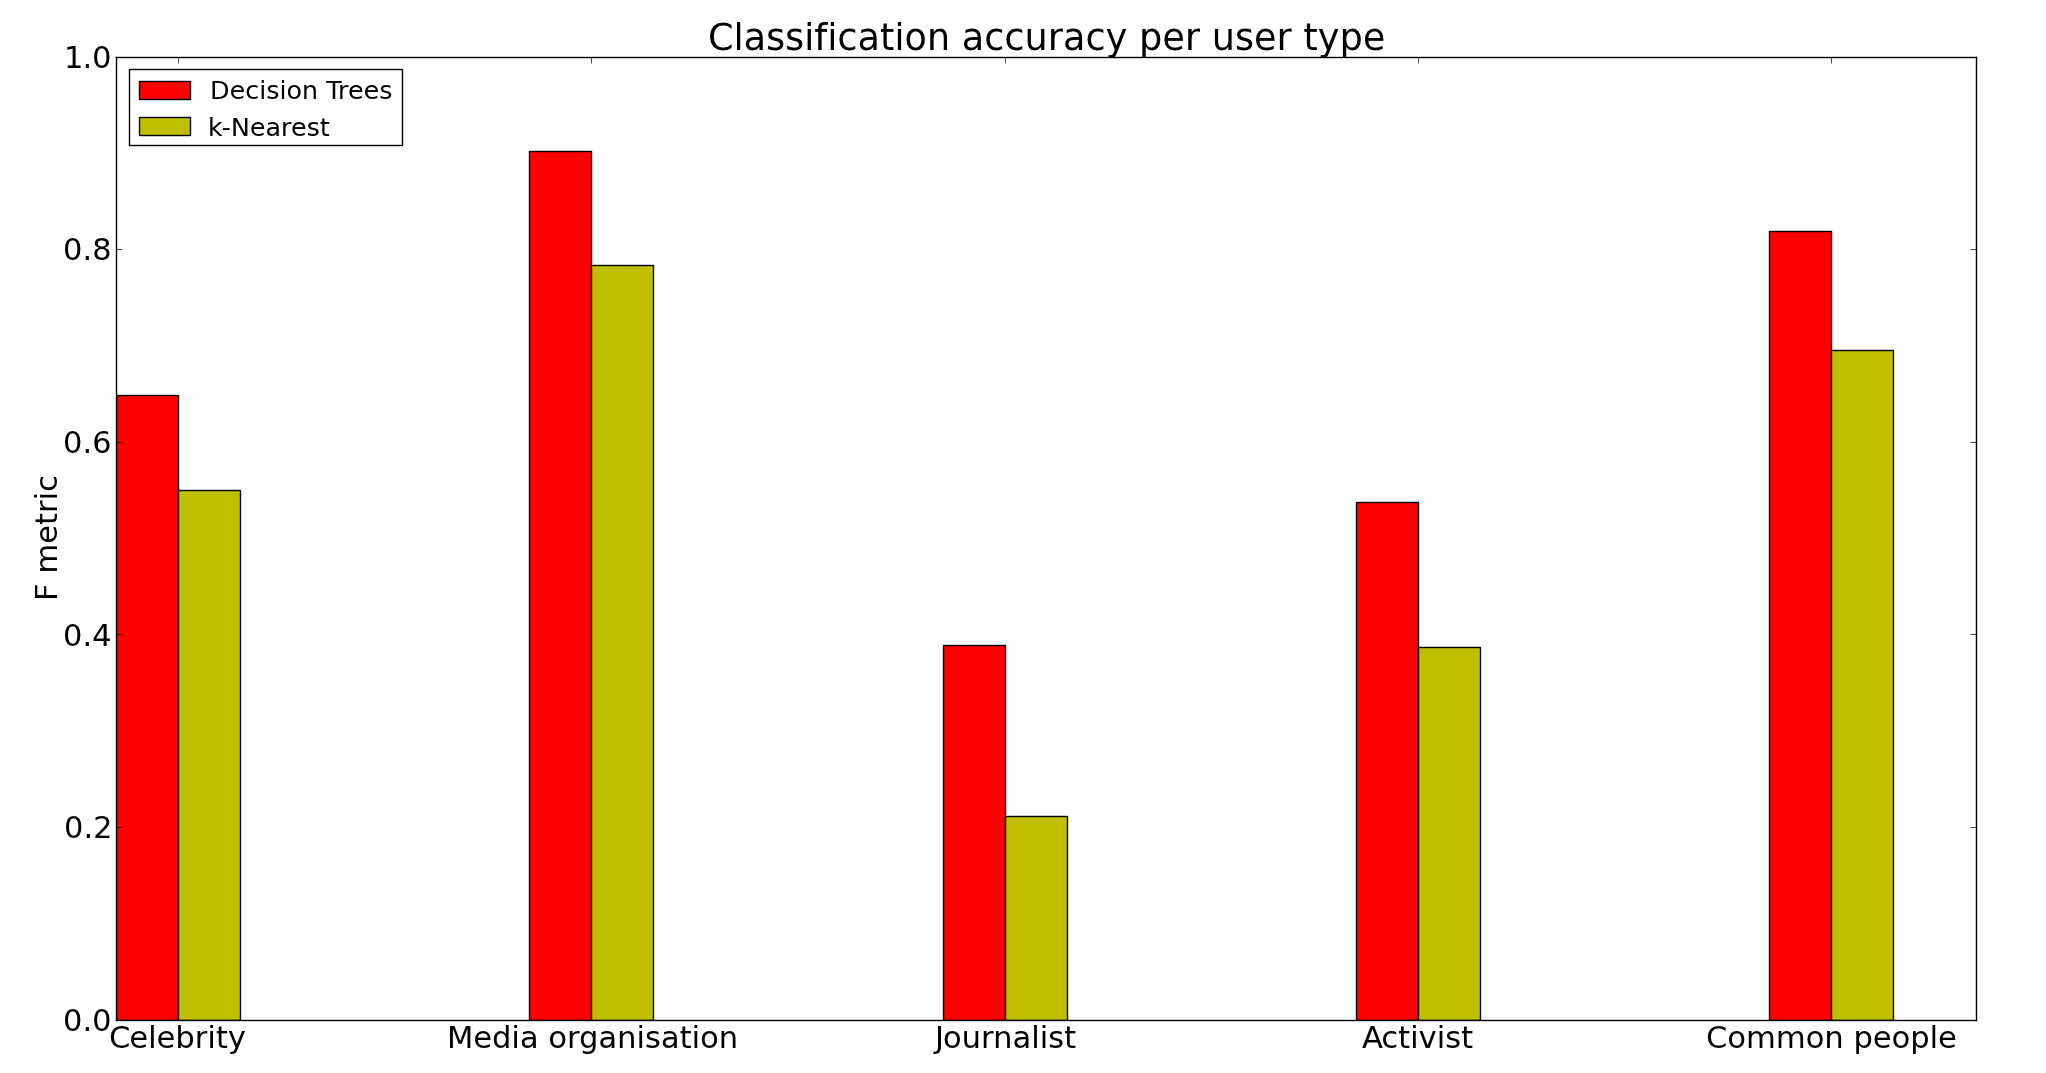
\includegraphics[height=5in, width=6in]{classifiers}
    \caption{The F metrics obtain after 10-fold cross validation on our dataset for the two classifiers.}
    \label{DifferentClassifiersResultsImproved}
  \end{center}
\end{figure}
A very important observation is the fact that for both classifiers the two classes with the lowest F score are the journalists and activists. This was expected because these two classes overlap significantly. Even for a human is difficult to distinguish between a journalist and an activist since sometimes some journalists are also activists. Finally, media organisations have the highest F score and again this was expected because they have some discriminating characteristics which can easily separate them from the other classes. Since these accounts act on behalf of huge organisations they do not act as humans but more like a bot. For example, they almost never engage in conversation nor they retweet.  


\section{Summary}
In this chapter we have evaluated and summarised our work related to clustering and classification algorithms. We have evaluated
clustering based on three different challenges of Twitter data and presented our results for our four clusterers. The results showed that 
two of the four algorithms outperformed the others in general. k-Means and DBSCAN were the best performing algorithms and the best performing similarity measure
was the cosine similarity. The other two algorithms had lower performance, with NMF being almost unable to produce clusters of acceptable performance. The online cluster
had lower performance than DBSCAN and k-Means and this was expected due to the trade-off between clustering quality and time performance. Even though, its performance was lower, in some cases
the results were promising indicating that there is room for improvement. \\\\
For classification the results were clearer indicating that the ID3 classifier was consistently better than k-Nearest neighbour at classifying unknown examples. The results of this chapter will guide our 
decisions in the next chapter when we present Pythia, a web application for event detection and summarisation. The best algorithms identified in this section will be used in the final implementation of Pythia.  
% ------------------------------------------------------------------------


%%% Local Variables: 
%%% mode: latex
%%% TeX-master: "../thesis"
%%% End: 
